\documentclass{beamer} 
\usetheme{default} 
\setbeamercovered{transparent}

%\useoutertheme{umbcfootline} 
\setbeamertemplate{background canvas}[vertical shading][bottom=red!20,top=yellow!30] 


\usepackage[spanish]{babel}
%\usepackage[latin1]{inputenc}
\usepackage[utf8x]{inputenc}
\usepackage{multicol}
\usepackage{color}


\title{Interfaces gráfica en Java}

\author{Manuel J. Molino Milla \and Luis Molina Garzón}

\date{\today} %

\institute{IES Virgen del Carmen \and Departamento de Informática}




%\beamerdefaultoverlayspecification{<+->}

\begin{document}


\begin{frame}
  \titlepage
\end{frame}

\begin{frame}
    \frametitle{Logo}
\begin{figure}

\includegraphics[scale=1]{imagenes/logo.jpeg} 
\caption{Logo Java}
\end{figure}
\end{frame}

\begin{frame}
  \frametitle{Contenido}
  \tableofcontents[pausesections]
\end{frame}



\section{Introduccion}

\begin{frame}
\frametitle{Interfaces gráficas}
\begin{quote}
La interfaz gráfica de usuario, conocida también como GUI (del inglés graphical user interface), es un programa informático que actúa de interfaz de usuario, utilizando un conjunto de imágenes y objetos gráficos para representar la información y acciones disponibles en la interfaz. 
\end{quote}
%\pause


\end{frame}
\begin{frame}
\frametitle{Interfaces gráficas}
\begin{figure}
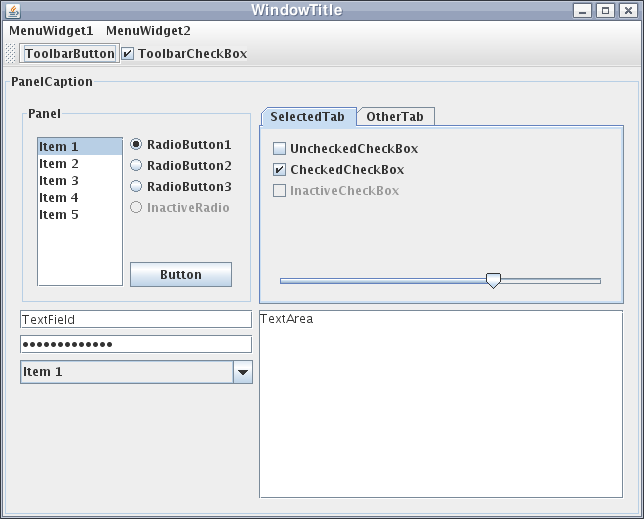
\includegraphics[scale=0.4]{imagenes/gui1.png}
\end{figure}
\end{frame}

\begin{frame}
\frametitle{API Java}
\begin{itemize}[<+->]
\item AWT
\item Swing
\item SWT
\item JavaFX
\end{itemize}
\end{frame}

\begin{frame}
\frametitle{Swing frente a AWT}
\begin{itemize}[<+->]
\item Las clases para la realización de interfaces gráfica (\alert{GUI}) fueron introducidas en una biblioteca conocida como \alert{AWT}
\item \emph{AWT} es acrónimo de \emph{Abstract Windows Toolkit}
\item AWT está muy bien para el desarrollo de interfaces gráficas de usuario sencillas, pero no para desarrollo de grandes proyectos.
\item Hoy en día se usa \alert{swing}. En la que todas las clases heredan de AWT.
\item Las clases de swing son fácilmente identificables pues empiezan con la letra \alert{J}, ejemplo \emph{JButton, JTextField, JTextArea, \dots}
\item Las API de GUI se pueden clasificar en tres grupos:
\begin{description}
\item[clases componentes] como \emph{JButton, JLabel, y JTextField}
\item[clases contenedoras] como \emph{JFrame, JPanel, y JApplet}
\item[clases ayudantes] como \emph{Graphics, Color, Font, FontMetrics, y Dimension}
\end{description}
\end{itemize}
\end{frame}

\begin{frame}
\frametitle{AWT y swing}
\begin{figure}
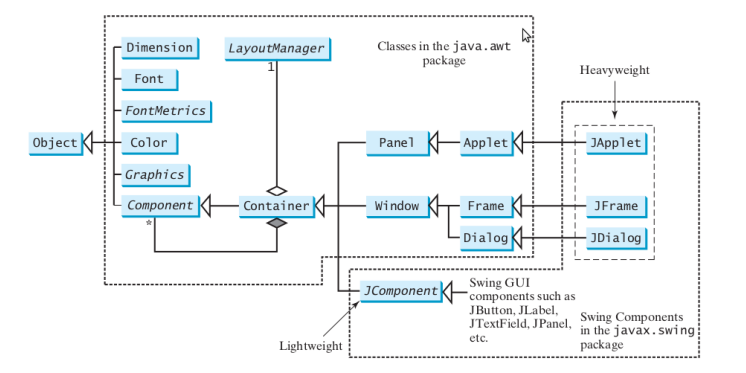
\includegraphics[width=\textwidth]{imagenes/awt_swing.png}
\caption{Java GUI}
\end{figure}
\end{frame}

\begin{frame}
\frametitle{Características de Swing}
\begin{itemize}[<+->]
\item Escrito totalmente en java.
\item No reemplaza a AWT.
\item Se apoya sobre AWT y añade JComponents.
\item Usa el modelo de eventos de java 1.1.
\item Selección de diferentes apariencias (Look and Feel).
\item Utilización de componentes ligeros (ligthweight) independientes del sistema operativo.
\item Arquitectura Modelo-Vista-Controlador (MVC).
\item Nuevos componentes (árboles, tablas, frames internos, etc.).
\end{itemize}
\end{frame}


\section{Clases contenedoras}

\begin{frame}
\frametitle{Introducción}
Existen dos elementos básicos para la creación de interfaces gráficas de usuario usando Swing:
\begin{description}[<+->]
\item[Contenedores:]Elementos capaces de albergar otros elementos. Ejemplo JFrame, JDialog o JApplet.
\item[Componentes:]Elementos que se añaden a contenedores. Ejemplo botones, áreas o caja de texto, \dots
\end{description}
\end{frame}




\begin{frame}
\frametitle{Clases contenedoras de alto nivel}
\begin{description}[<+->]
\item[JFrame] Es una ventana que no está contenida dentro de otra ventana. Es la mas usada en GUI de tipo swing. Se visualiza como una ventana principal con marco y barra de título.
\item[JApplet] Permite crear aplicaciones con interface gráfica que se ejecutan en el contexto de un navegador web.
\item[JDialog] Se visualiza como una ventana independiente de la ventana principal para mostrar información, como por ejemplo el contenido de un directorio.
\end{description}
\end{frame}


\subsection{JFrame}
\begin{frame}[fragile]
\frametitle{JFrame}
\begin{small}
\begin{verbatim}
import javax.swing.JFrame;
public class PrimeraFrame
{

  public static void main (String[]args)
  {
    //creamos la frame
    JFrame frame = new JFrame ("Primera Frame");
      frame.setSize (400, 300); // Tamaño
      frame.setLocationRelativeTo (null); // Centramos
      //permitimos el cierre
      frame.setDefaultCloseOperation (JFrame.EXIT_ON_CLOSE);
      frame.setVisible (true);  // Display la frame
  }
}
\end{verbatim}
\end{small}
\end{frame}


\begin{frame}
\frametitle{JFrame} 
\begin{multicols}{2}
\begin{figure}
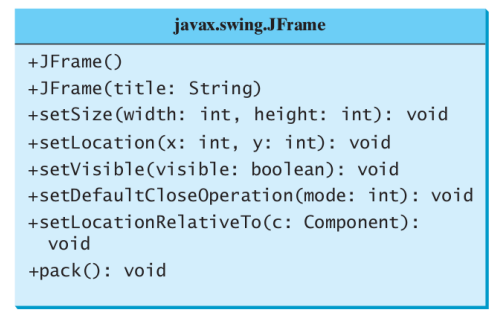
\includegraphics[scale=0.4]{imagenes/frame.png}
\end{figure}
\begin{enumerate}[<+->]
\item Crea una frame sin título.
\item Crea una frame con título.
\item Establece el tamaño de la frame.
\item Establece la posición de la esquina superior izquierda.
\item Hace visible la frame.
\item Establece la operación ha realizar cuando se cierra la frame.
\item Establece la posición relativa de la frame a algún componente. En caso de null queda centrada.
\item Establece el tamaño según los componentes de la frame.
\end{enumerate}
\end{multicols}

\end{frame}



\begin{frame}[fragile]
    \frametitle{Añadir componentes a la frame}
\begin{footnotesize}
\begin{itemize}[<+-| alert@+>]
      \item Ahora mismo la frame esta vacia, hay que añadir componentes:
        
\end{itemize}
\begin{verbatim}
import javax.swing.*;
public class FrameConBoton
{
  public static void main (String[]args)
  {
    JFrame frame = new JFrame ("Primera Frame");// crea una frame
// Añadimos un boton a la frame
    JButton jbtOK = new JButton ("OK");
    frame.add (jbtOK);
    frame.setSize (400, 300); // Tamaño
    frame.setLocationRelativeTo (null);       // Centra
    frame.setDefaultCloseOperation (JFrame.EXIT_ON_CLOSE);//cierre
    frame.setVisible (true);  // Display la frame
  }
}
\end{verbatim}

\pause
En versiones anteriores de Java, había que usar el método \emph{getContentPane} para obtener el contenido del panel y posteriormente colocar el componente:\\
\alert{java.awt.Container container = frame.getContentPane();}\\
\alert{container.add(jbtOK);}
\end{footnotesize}
\end{frame}


\begin{frame}
\frametitle{Componentes}
Una vez que hemos creado un contenedor, los componentes los añadiremos siguiendo las siguiente reglas:
\begin{itemize}[<+->]
\item Un componente se visualizará si lo hemos añadido a un contenedor.
\item Un componente sólo se puede añadir una vez a un contenedor.
\item Los componentes los debemos añadir al panel del contenedor.
\end{itemize}
\end{frame}

\begin{frame}
\frametitle{Estructura de un JFrame}
\begin{figure}
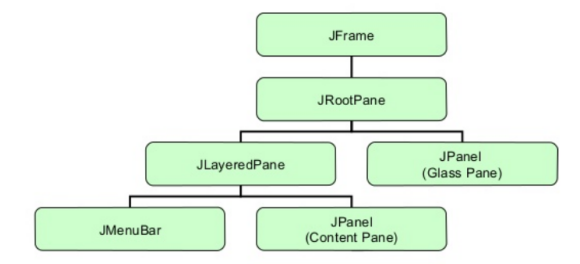
\includegraphics[scale=0.4]{imagenes/arq_swing.png}
\end{figure}
\begin{description}[<+->]
\item[JFrame] es la ventana principal
\item[JRootPane] contenedor principal
\item[JLayaredPane] panel de capas, contiene la barra de menu y permite añadir componentes al panel
\item[JMenuBar] presenta la barra de menu superior.
\item[Conte Pane] para añadir componentes
\item[Panel transparente] para acciones de \emph{drag and drop}
\end{description}
\end{frame}

\begin{frame}
\frametitle{Estructura de un JFrame}
\begin{figure}
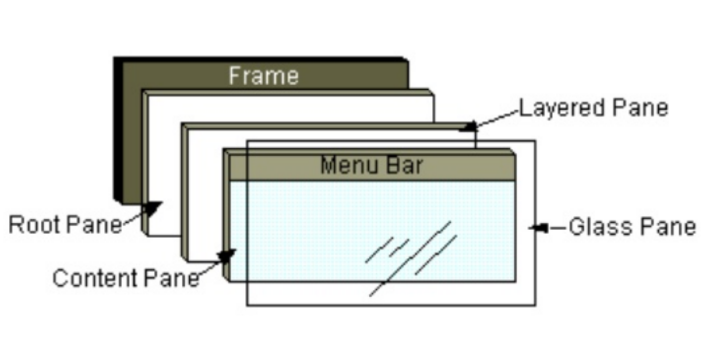
\includegraphics[scale=0.6]{imagenes/arq1_swing.png}
\end{figure}
\end{frame}

\begin{frame}
\frametitle{Implementación óptima}
\begin{figure}
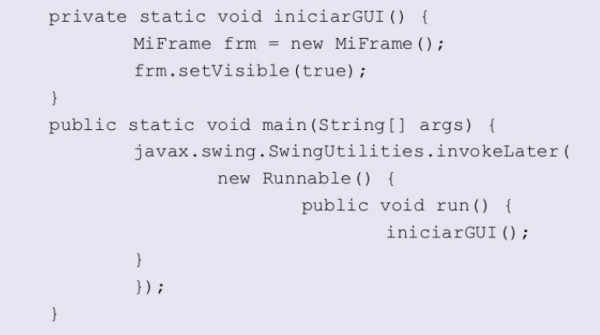
\includegraphics[scale=0.5]{imagenes/invokelater.png}
\end{figure}
La gestión de eventos y el pintado/repintado de la GUI se hace desde un hilo independiente. En el caso que algún componente va a durar mucho se debe realizar en un hilo aparte. De esta manera evitaremos posteriores problemas con el manejador de eventos cuando acabe dicha tarea.
\end{frame}

\section{Layout}
\begin{frame}[fragile]
    \frametitle{Layaout}
  \begin{itemize}[<+->]
  \item Hasta ahora estamos disponiendo los componentes en la interfaz usando una posición absoluta en píxeles.
  \item Puede ocurrir, que de esta manera, sean correctamente dispuestos en un sistema, pero no en otro.
  \item Java permite un nivel de abstración que se encarga de la colocación de los componentes en los contenedores, denominada \alert{layaout}
  \item En este caso no se especifica donde colocar los componentes y es el layaout quien se encarga de esto.
  \item Para esto usamos la clase \alert{LayoutManager}:
    \end{itemize}
    \pause
    \begin{quote}
    LayoutManager layoutManager = new XLayout();\\
container.setLayout(layoutManager);
    \end{quote}
    \pause
    Donde \emph{layaoutManager} puede ser \alert{FlowLayout, GridLayout, BorderLayout, CardLayout, GroupLayout}\\
  \begin{center}
  {\color{blue}\href{https://docs.oracle.com/javase/tutorial/uiswing/layout/visual.html}{Guia de layouts en swing}}
  \end{center}
    
\end{frame}



\subsection{FlowLayout}
\begin{frame}
    \frametitle{FlowLayout}
\begin{itemize}[<+->]
\item Es el layout mas simple.
\item Los componentes se añaden de izquierda a derecha a medida que se van agregrando.
\item Se puede establecer la alineación de los componentes con \alert{FlowLayout.RIGHT, FlowLayout.CENTER, o FlowLayout.LEFT.}
\item \emph{hgap} controla la separación horizontal de los componentes
\item \emph{vgap} idem pero la disposción vertical.
\item Se usan \emph{setters} para estas acciones.
\end{itemize}
\end{frame}


\begin{frame}[fragile]
    \frametitle{FlowLayout}
    \begin{multicols}{2}
\begin{tiny}
\begin{verbatim}
import java.awt.FlowLayout;
import javax.swing.*;
public class PrimerLayout extends JFrame
{
  public PrimerLayout ()
  {
//espacido 10 y 20 pixeles entre componentes
    setLayout (new FlowLayout (FlowLayout.LEFT, 10, 20));
    add (new JLabel ("Etiqueta"));
    add (new JTextField (8));
    add (new JLabel ("MI"));
    add (new JTextField (1));
    add (new JLabel ("Otra etiqueta"));
    add (new JTextField (8));
  }
  public static void main (String[]arg)
  {
    PrimerLayout frame = new PrimerLayout ();
    frame.setTitle ("Frame con FlowLayout");
    frame.setSize (200, 200);   // Tamaño
    frame.setLocationRelativeTo (null); // Centra
    frame.setDefaultCloseOperation (JFrame.EXIT_ON_CLOSE);      //cierre
    frame.setVisible (true);    // Display la frame
  }
}
\end{verbatim}
\end{tiny}
\begin{figure}
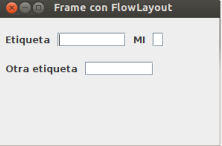
\includegraphics[scale=0.7]{imagenes/primerlayout.png}
\end{figure}
\end{multicols}
\end{frame}

\begin{frame}[fragile]
    \frametitle{FlowLayaout}
  \begin{itemize}[<+->]
  \item Si redimensionamos la frame, los componentes se ajustan automáticamente.
  \item En \alert{setLayout(new FlowLayout(FlowLayout.LEFT, 10, 20) );} estamos definiendo un objeto anónimo de la clase FlowLayout.
  \item Esto es equivalente a:
  \end{itemize}
  \pause
  \begin{quote}
  FlowLayout layout = new FlowLayout(FlowLayout.LEFT, 10, 20);\\
  setLayout(layout);

  \end{quote}
\end{frame}

\begin{frame}[fragile]
    \frametitle{FlowLayaout}
  \begin{figure}
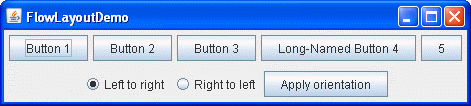
\includegraphics[scale=0.7]{imagenes/fl.png}
\end{figure}  
\begin{center}
{\color{blue}\href{https://docs.oracle.com/javase/tutorial/displayCode.html?code=https://docs.oracle.com/javase/tutorial/uiswing/examples/layout/FlowLayoutDemoProject/src/layout/FlowLayoutDemo.java}
{Codigo de la interfaz}}
\end{center}
\end{frame}

\subsection{GridLayout}
\begin{frame}[fragile]
\frametitle{GridLayout}
\begin{itemize}[<+->]
\item Divide el contenedor en una cuadrícula. 
\item Los componentes se colocan de izquierda a derecha empezando por la primera fila.
\item Se puede especificar el número de filas y columnas.
\item Puede ser cero el número de filas o cero el número de columnas. Pero no las dos.
\item Si una es cero, por ejemplo en filas y tenemos tres columnas, si añadimos cinco componentes, tendremos dos filas (2 x 3).
\item En el caso que fijemos una cuadrícula de 3 x 3 (9), y ponemos diez componentes, se crean tres filas y cuatro columnas.
\item La redimensión de la ventana no varía la estructura.
\end{itemize}
\end{frame}


\begin{frame}[fragile]
\frametitle{GridLayout}
\begin{multicols}{2}
\begin{tiny}
\begin{verbatim}
import java.awt.GridLayout;

import javax.swing.*;
public class PrimerGridLayout extends JFrame
{
  public PrimerGridLayout ()
  {


//tres filas y dos columnases y 5 pixeles entre componentes
    setLayout (new GridLayout (3,2,5,5));
    add (new JLabel ("Etiqueta"));
    add (new JTextField (8));
    add (new JLabel ("MI"));
    add (new JTextField (1));
    add (new JLabel ("Otra etiqueta"));
    add (new JTextField (8));
  }
  public static void main (String[]arg)
  {

    PrimerGridLayout frame = new PrimerGridLayout ();
    frame.setTitle ("Frame con GridLayout");
    frame.setSize (200, 200);   // Tamaño
    frame.setLocationRelativeTo (null); // Centra
    frame.setDefaultCloseOperation (JFrame.EXIT_ON_CLOSE);//cierre
    frame.setVisible (true);    // Display la frame
  }
}
\end{verbatim}
\end{tiny}

\begin{figure}
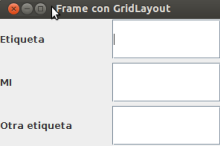
\includegraphics[scale=0.64]{imagenes/gridlayout.png}
\end{figure}
\end{multicols}
\end{frame}

\begin{frame}[fragile]
    \frametitle{GridLayaout}
  \begin{figure}
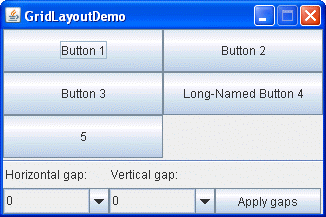
\includegraphics[scale=0.7]{imagenes/gridl.png}
\end{figure}  
\begin{center}{\color{blue}
\href{https://docs.oracle.com/javase/tutorial/displayCode.html?code=https://docs.oracle.com/javase/tutorial/uiswing/examples/layout/GridLayoutDemoProject/src/layout/GridLayoutDemo.java}{Codigo de la interfaz}}
\end{center}
\end{frame}

\subsection{BorderLayout}
\begin{frame}[fragile]
    \frametitle{BorderLayout}
       \begin{itemize}[<+->]
       \item Divide el contenedor en cinco áreas:
       \begin{enumerate}
\item East
\item South
\item West
\item North,
\item Center
\end{enumerate}
\item Los componentes se añaden con \alert{add(Component,index)} donde  index es una constante:
\begin{enumerate}
\item BorderLayout.EAST
\item BorderLayout.SOUTH
\item BorderLayout.WEST
\item BorderLayout.NORTH
\item BorderLayout.CENTER.
\end{enumerate}
\item ¿Qué ocurrirá si no se pone alguna área?
       \end{itemize}
 
\end{frame}

\begin{frame}[fragile]
\frametitle{BorderLayout}
\begin{multicols}{2}
\begin{tiny}
\begin{verbatim}
import java.awt.BorderLayout;

import javax.swing.*;
public class PrimerBorderLayout extends JFrame
{
  public PrimerBorderLayout ()
  {

//Separación de  5 y 10 pixeles entre componentes
    setLayout (new BorderLayout (5, 10));

    add (new JButton ("East"), BorderLayout.EAST);
    add (new JButton ("South"), BorderLayout.SOUTH);
    add (new JButton ("West"), BorderLayout.WEST);
    add (new JButton ("North"), BorderLayout.NORTH);
    add (new JButton ("Center"), BorderLayout.CENTER);

  }
  public static void main (String[]arg)
  {

    PrimerBorderLayout frame = new PrimerBorderLayout ();
    frame.setTitle ("Frame con BorderLayaout");
    frame.setSize (300, 200);   // Tamaño
    frame.setLocationRelativeTo (null); // Centra
    frame.setDefaultCloseOperation (JFrame.EXIT_ON_CLOSE);      //cierre
    frame.setVisible (true);    // Display la frame
  }
}
\end{verbatim}
\end{tiny}
\begin{figure}
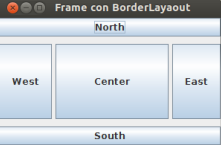
\includegraphics[scale=0.6]{imagenes/borderlayout.png}
\end{figure}
\end{multicols}
\end{frame}


\begin{frame}[fragile]
    \frametitle{BorderLayaout}
  \begin{figure}
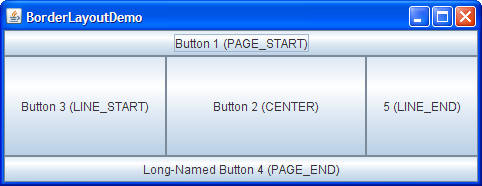
\includegraphics[scale=0.7]{imagenes/bl.png}
\end{figure}  
\begin{center}{\color{blue}
\href{https://docs.oracle.com/javase/tutorial/displayCode.html?code=https://docs.oracle.com/javase/tutorial/uiswing/examples/layout/BorderLayoutDemoProject/src/layout/BorderLayoutDemo.java}
{Codigo de la interfaz}}
\end{center}
\end{frame}

\subsection{BoxLayout}

\begin{frame}[fragile]
    \frametitle{BoxLayout}
\begin{itemize}[<+->]
\item Ubica los componentes tanto de forma vertical u horizontal
\item Similar a \emph{FlowLayout}, pero éste solo los coloca de forma horizontal
\item Para crear una clase \emph{BoxLayout}, necesitamos dos argumentos.
\end{itemize}
\pause
\begin{block}{Horizontal}
\begin{verbatim}
JFrame frame = new JFrame();
frame.setLayout(new BoxLayout(frame,BoxLayout.X_AXIS));
\end{verbatim}
\end{block}
\pause
\begin{block}{Vertical}
\begin{verbatim}
JFrame frame = new JFrame();
frame.setLayout(new BoxLayout(frame,BoxLayout.Y_AXIS));
\end{verbatim}
\end{block}
\end{frame}

\begin{frame}[fragile]
    \frametitle{BoxLayaout}
  \begin{figure}
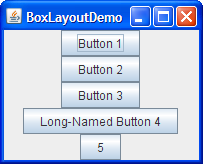
\includegraphics[scale=0.7]{imagenes/bl1.png}
\end{figure}  
\begin{center}{\color{blue}
\href{https://docs.oracle.com/javase/tutorial/displayCode.html?code=https://docs.oracle.com/javase/tutorial/uiswing/examples/layout/BoxLayoutDemoProject/src/layout/BoxLayoutDemo.java}
{Codigo de la interfaz}}
\end{center}
\end{frame}


\begin{frame}[fragile]
    \frametitle{BoxLayaout}
  \begin{figure}
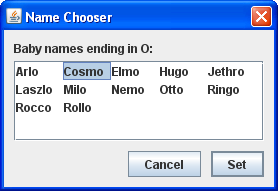
\includegraphics[scale=0.7]{imagenes/bl2.png}
\end{figure}  
\begin{center}{\color{blue}
\href{https://docs.oracle.com/javase/tutorial/displayCode.html?code=https://docs.oracle.com/javase/tutorial/uiswing/examples/components/ListDialogRunnerProject/src/components/ListDialog.java}
{Codigo de la interfaz}}
\end{center}
\end{frame}


\subsection{CardLayout}
\begin{frame}[fragile]
    \frametitle{CardLayout}
\begin{itemize}[<+->]
\item CardLayout,  es un manejador de diseño que nos permite, ubicar componentes swing dentro de un mismo contenedor, y poder visualizarlos solamente uno a la vez.
\item Tenemos un contenedor pricipal, y dentro de el, varios paneles, y a través de una seleccion, elegir cual de estos paneles queremos visualizar.
\end{itemize}
\pause
\begin{block}{Creamos el contenedor y agregamos los componentes}
\begin{verbatim}
JFrame frame = new JFrame();
frame.setLayout(new CardLayout());
JPanel panel = new JPanel();
JPanel pane2 = new JPanel();
frame.add(panel, referenciaPanel1);
frame.add(pane2, referenciaPanel2);
\end{verbatim}
\end{block}
\end{frame}

\begin{frame}
\frametitle{CardLayout}
\begin{block}{Metodos importantes}
\begin{description}
\item[first (nombreContenedor)] Visualizamos el primer objeto añadido
\item[next (nombreContenedor)] Visualizamos el segundo objeto añadido
\item[previous (nombreContenedor)] Visualizmaos el objeto anterior
\item[show (nombreContenedor, referenciaPanel) ] visualiza el contenedor de la referencia.
\end{description}
\end{block}

\end{frame}

\begin{frame}[fragile]
    \frametitle{CardLayaout}
  \begin{figure}
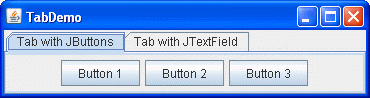
\includegraphics[scale=0.7]{imagenes/cl.png}
\end{figure}  
\begin{center}{\color{blue}
\href{https://docs.oracle.com/javase/tutorial/displayCode.html?code=https://docs.oracle.com/javase/tutorial/uiswing/examples/layout/TabDemoProject/src/layout/TabDemo.java}
{Codigo de la interfaz}}
\end{center}
\end{frame}




\subsection*{Combinacion de layaouts}

\begin{frame}
    \frametitle{ComposiciónCombinacion de layaouts}
\begin{itemize}[<+->]
\item Los layouts que hemos visto estan muy limitados.
\item Se pueden combinar layaouts. 
\item Ejemplo:
\end{itemize}
\pause
\begin{figure}
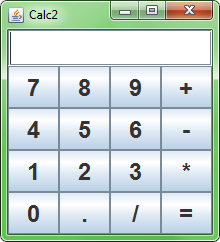
\includegraphics[scale=0.5]{imagenes/calculadora.png}
\end{figure}
\pause
\begin{itemize}[<+->]
\item Se puede conseguir von un BorderLayout en el norte con un TextField
\item Un GridLayout de 4 x 4, con un Button en cada celda.
\end{itemize}
\end{frame}



\begin{frame}[fragile]
\frametitle{Chat}
¿Como hariamos este Chat?
\begin{figure}
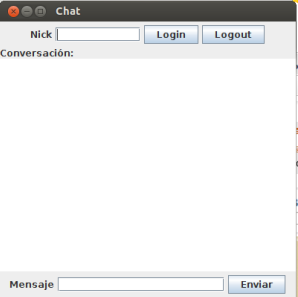
\includegraphics[scale=0.7]{imagenes/chat.png}
\end{figure}
\end{frame}


\section*{Color}
\begin{frame}[fragile]
\frametitle{Clase java.awt.Color}
\begin{itemize}[<+->]
\item Podemos crear colores con el siguiente constructor:
\item \alert{public Color (int r, int g, int b)}
\item Donde \alert{r,g,b} representa la intensidad de color del rojo, verde y azul respectivamente.
\item El rango de valor va desde \emph{0 a 255}
\item Ejemplo:
\item Color color = new Color(128, 100, 100);
\item Alternativamente se pueden usar 13 colores estándar: \emph{BLACK, BLUE, CYAN, DARK\_GRAY, GRAY, GREEN, LIGHT\_GRAY, MAGENTA, ORANGE, PINK, RED, WHITE y YELLOW}
\item También se puede usar los métodos \alert{setBackground(Color c)} para el color de fondo.
\item Y \alert{setForeground(Color c)} para el color de la fuente.
\end{itemize}
\end{frame}



\begin{frame}[fragile]
\frametitle{Ejemplo Color}
\begin{tiny}
\begin{verbatim}
import java.awt.BorderLayout;
import java.awt.Color;

import javax.swing.*;
public class PrimerBorderLayoutColor extends JFrame
{
  public PrimerBorderLayoutColor ()
  {

//Separación de  5 y 10 pixeles entre componentes
    setLayout (new BorderLayout (5, 10));
    Color color = new Color (128, 100, 100);
    JButton este = new JButton ("East");
      este.setBackground (color);
    JButton oeste = new JButton ("West");
      oeste.setForeground (new Color (255, 0, 0));

      add (este, BorderLayout.EAST);
      add (new JButton ("South"), BorderLayout.SOUTH);
      add (oeste, BorderLayout.WEST);
      add (new JButton ("North"), BorderLayout.NORTH);
      add (new JButton ("Center"), BorderLayout.CENTER);

  }
  public static void main (String[]arg)
  {

    PrimerBorderLayoutColor frame = new PrimerBorderLayoutColor ();
    frame.setTitle ("Frame con BorderLayaout");
    frame.setSize (300, 200);   // Tamaño
    frame.setLocationRelativeTo (null); // Centra
    frame.setDefaultCloseOperation (JFrame.EXIT_ON_CLOSE);      //cierre
    frame.setVisible (true);    // Display la frame
  }
}
\end{verbatim}
\end{tiny}
\end{frame}

\begin{frame}
\frametitle{Ejemplo Color} 
\begin{figure}
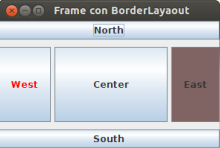
\includegraphics[scale=0.9]{imagenes/color.png} 
\end{figure} 
\end{frame}

\section*{Font}
\begin{frame}[fragile]
\frametitle{java.awt.Font}
\begin{itemize}[<+->]
\item El constructor para \emph{Font} es:
\item \alert{public Font(String nombre, int estilo, int tamaño);}
\item Donde nombre puede ser: \emph{SansSerif, Serif, Monospaced, Dialog, o DialogInput}
\item Y estilo \emph{Font.PLAIN (0), Font.BOLD (1), Font.ITALIC (2), y Font.BOLD + Font.ITALIC (3)}
\item Ejemplo:
\item \emph{Font font1 = new Font(''SansSerif'', Font.BOLD, 16);}
\item \emph{Font font2 = new Font(''Serif'', Font.BOLD + Font.ITALIC, 12);}
\end{itemize}
\end{frame}

\begin{frame}[fragile]
\frametitle{Ejemplo Font}
\begin{tiny}
\begin{verbatim}
import java.awt.BorderLayout;
import java.awt.Font;

import javax.swing.*;
public class PrimerBorderLayoutFont extends JFrame
{
  public PrimerBorderLayoutFont ()
  {

//Separación de  5 y 10 pixeles entre componentes
    setLayout (new BorderLayout (5, 10));
    Font font1 = new Font ("SansSerif", Font.BOLD, 16);
    Font font2 = new Font ("Serif", Font.BOLD + Font.ITALIC, 12);
    JButton este = new JButton ("East");
      este.setFont (font1);
    JButton oeste = new JButton ("West");
      oeste.setFont (font2);

      add (este, BorderLayout.EAST);
      add (new JButton ("South"), BorderLayout.SOUTH);
      add (oeste, BorderLayout.WEST);
      add (new JButton ("North"), BorderLayout.NORTH);
      add (new JButton ("Center"), BorderLayout.CENTER);
  }
  public static void main (String[]arg)
  {
    PrimerBorderLayoutFont frame = new PrimerBorderLayoutFont ();
    frame.setTitle ("Frame con BorderLayaout");
    frame.setSize (300, 200);   // Tamaño
    frame.setLocationRelativeTo (null); // Centra
    frame.setDefaultCloseOperation (JFrame.EXIT_ON_CLOSE);      //cierre
    frame.setVisible (true);    // Display la frame
  }
}
\end{verbatim}
\end{tiny}
\end{frame}

\begin{frame}
\frametitle{Ejemplo Font} 
\begin{figure}
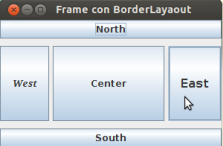
\includegraphics[scale=0.9]{imagenes/font.png} 
\end{figure} 
\end{frame}

\section*{Imagenes}
\begin{frame}[fragile]
\frametitle{javax.swing.ImageIcon}
\begin{itemize}[<+->]
\item Java soporta tres tipos de imágenes \emph{png, jpg y gif}
\item Se usa un objeto de tipo \alert{ImageIcon}
\item Ejemplo:
\item \emph{ImageIcon icon = new ImageIcon(''imagenes/us.gif'');}
\item Una imagen se puede colocar en una etiqueta o en un boton:
\item \alert{new JLabel(imagen)}
\item \alert{new JButton(imagen)}
\end{itemize}
\end{frame}

\begin{frame}[fragile]
\frametitle{Imágenes}
\begin{multicols}{2}
\begin{figure}
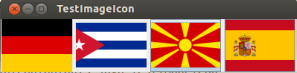
\includegraphics[scale=0.5]{imagenes/imagen.png}
\end{figure}
\begin{tiny}
\begin{verbatim}
import javax.swing.*;
import java.awt.*;
public class TestImageIcon extends JFrame
{
  private ImageIcon alIcon =
       new ImageIcon ("imagenes/alemania.png");
  private ImageIcon cuIcon = 
       new ImageIcon ("imagenes/cuba.png");
  private ImageIcon maIcon = 
       new ImageIcon ("imagenes/macedonia.png");
  private ImageIcon esIcon = 
       new ImageIcon ("imagenes/espana.png");
  
  
  public TestImageIcon ()
  {
    setLayout (new GridLayout (1, 4, 5, 5));
    add (new JLabel (alIcon));
    add (new JLabel (cuIcon));
    add (new JButton (maIcon));
    add (new JButton (esIcon));
  }
  public static void main (String[]args)
  {
    TestImageIcon frame = new TestImageIcon ();
    frame.setTitle ("TestImageIcon");
    frame.setSize (400, 100);
    frame.setLocationRelativeTo (null); // Center the frame
    frame.setDefaultCloseOperation (JFrame.EXIT_ON_CLOSE);
    frame.setVisible (true);
  }
}
\end{verbatim}
\end{tiny}
\end{multicols}
\end{frame}

\begin{frame}
\frametitle{Preguntas} 
\begin{figure}

\includegraphics[scale=0.9]{imagenes/dudas.png} 
\end{figure} 
\end{frame}

\end{document}

